\section{Experiments}
\label{sec:experiments}

% All tables in this section are generated by `python aggregate.py` from the result files
% (paper/tables/*.tex); do not edit numbers by hand.

\subsection{Setup}
\label{sec:setup}

\paragraph{Data and models.} We use CIFAR-10 and CIFAR-100 \cite{krizhevsky2009learning} with per-channel normalisation, random cropping (padding 4) and horizontal flipping. ResNet-18 \cite{he2016deep} is used in its CIFAR form (3$\times$3 stem, no initial pooling; 11.2M conv/linear weights). VGG-16 with BatchNorm \cite{simonyan2015very} uses the same CIFAR conventions and a global average pool before the classifier.

\paragraph{Training.} Every run uses the same recipe (Table~\ref{tab:hyperparams}): SGD with momentum 0.9, weight decay $5\times10^{-4}$, batch size 128, 200 epochs, learning rate 0.1 with cosine decay, bfloat16 autocast, in PyTorch \cite{paszke2019pytorch}. No hyper-parameter was tuned for any criterion. We report the \emph{final-epoch} test accuracy; the test set is evaluated every 10 epochs for monitoring only and is never used for selection. Dense references use one seed and serve as a ceiling, not as a tested arm.

\begin{table}[t]
\centering
\caption{Training and loop hyper-parameters, identical for every criterion.}
\label{tab:hyperparams}
\begin{tabular}{lc}
\toprule
\multicolumn{2}{c}{Training} \\
\midrule
Epochs & 200 \\
Batch size & 128 \\
Optimiser & SGD, momentum 0.9 \\
Learning rate & 0.1, cosine decay \\
Weight decay & $5\times10^{-4}$ \\
Precision & bfloat16 autocast \\
Seeds & 3 (5 for $|w|$ and $H\cdot|w|$) \\
\midrule
\multicolumn{2}{c}{Prune-and-regrow loop} \\
\midrule
Warm-up $T_w$ & 10 epochs \\
Update interval $\Delta T$ & 400 iterations \\
Update fraction $\alpha$ & 0.2, cosine decay \\
Update end $T_{\text{end}}$ & epoch 150 \\
Regrowth & dense gradient magnitude \\
Allocation & global, 1\% per-layer floor \\
Entropy bins $B$ / batches $K$ & 30 / 4 \\
\bottomrule
\end{tabular}
\end{table}

\paragraph{Hardware and cost.} All runs were made on one NVIDIA GeForce RTX 3090 (driver 595.84). \TODO{Add CUDA runtime and PyTorch versions from the training environment.} A ResNet-18 run takes about 7\,s per epoch and a VGG-16 run about 4.3\,s; the whole study took 36 GPU-hours. The entropy histograms take about 1\% of training time (1.0--1.1\% for ResNet-18, 0.8\% for VGG-16, 1.5\% for the robust estimate), and the topology updates 1.2\% for magnitude-type scores on ResNet-18 (2.0\% on VGG-16) and 3--4.6\% for Taylor, Fisher and $|g|$, whose statistics are accumulated at every step.

\subsection{The starting point: an ablation of the drop score}
\label{sec:c0}

Table~\ref{tab:c0} runs the loop with three drop scores and nothing else changed: $|w|$ (A), $H$ alone (B) and $H\cdot|w|$ (C). We had fixed in advance that entropy would count as useful only if C exceeded A by more than $1.96$ times the pooled standard deviation.

\begin{table*}[t]
\centering
\caption{Ablation C0: the same prune/regrow loop with three drop criteria (CIFAR-10, ResNet-18, 90\% target sparsity). Only the importance score differs between rows.}
\label{tab:c0}
\resizebox{\textwidth}{!}{%
\begin{tabular}{llccccc}
\toprule
Cfg & Drop score & Acc (\%) & Sparsity (\%) & FLOPs red.\ sparse (\%) & Non-zero weights & Seeds \\
\midrule
A & $|w|$ & 95.03 $\pm$ 0.07 & 90.00 $\pm$ 0.00 & 75.2 $\pm$ 1.5 & 1,116,435 $\pm$ 0 & 3 \\
B & $H(A)$ & 92.44 $\pm$ 0.40 & 90.00 $\pm$ 0.00 & 86.0 $\pm$ 0.7 & 1,116,435 $\pm$ 0 & 3 \\
C & $H(A)\cdot|w|$ & 95.30 $\pm$ 0.21 & 90.00 $\pm$ 0.00 & 73.6 $\pm$ 0.7 & 1,116,435 $\pm$ 0 & 3 \\
\bottomrule
\end{tabular}}
\par\smallskip\footnotesize Mean $\pm$ std over 3 seeds; $^{*}$ marks single-seed cells (no std); -- = not yet run. Accuracy is final-epoch test accuracy.
\end{table*}


C is $+0.27$ points above A, below the threshold of $0.31$ points, and B is $2.59$ points below A. A first run of the same ablation, made before the final version of the code, gave $-0.04$ and $-2.45$ points; the numbers in Table~\ref{tab:c0} come from a complete re-run with the code used for every other result, and both runs lead to the same decision. Entropy-weighted magnitude did not improve on magnitude, and entropy alone was clearly worse. This is the observation that motivated the study.

\subsection{Criteria across regimes}
\label{sec:results}

Table~\ref{tab:regimes} reports every criterion in every regime against $|w|$.

\begin{table*}[t]
\centering
\caption{Drop criteria inside one prune/regrow loop across regimes (global allocation). Only the drop score differs within a block; regrowth is by gradient magnitude in every row.}
\label{tab:regimes}
\resizebox{\textwidth}{!}{%
\begin{tabular}{llcccccc}
\toprule
Regime & Drop criterion & Acc (\%) & $\Delta$ vs $|w|$ [95\% CI] (pp) & $p_{\mathrm{Holm}}$ & Equiv. & FLOPs red.\ sparse (\%) & Seeds \\
\midrule
CIFAR-10, ResNet-18, 90\% & Dense & 95.34$^{*}$ &  &  &  & 0.0 & 1 \\
CIFAR-10, ResNet-18, 90\% & $|w|$ & 95.05 $\pm$ 0.19 & -- & -- & -- & 74.5 $\pm$ 1.5 & 5 \\
CIFAR-10, ResNet-18, 90\% & $H(A)$ & 92.44 $\pm$ 0.40 & -2.61 [-3.47, -1.74] & 0.041 & no & 86.0 $\pm$ 0.7 & 3 \\
CIFAR-10, ResNet-18, 90\% & $H(A)\cdot|w|$ (DEGST) & 95.26 $\pm$ 0.18 & +0.21 [-0.06, +0.48] & 0.881 & no & 73.4 $\pm$ 1.1 & 5 \\
CIFAR-10, ResNet-18, 90\% & Random (control) & 94.23 $\pm$ 0.35 & -0.82 [-1.55, -0.09] & 0.339 & no & 81.5 $\pm$ 1.2 & 3 \\
CIFAR-10, ResNet-18, 90\% & Taylor $|wg|$ & 94.99 $\pm$ 0.12 & -0.05 [-0.32, +0.22] & 1.000 & yes & 71.0 $\pm$ 2.5 & 3 \\
CIFAR-10, ResNet-18, 90\% & Fisher $(wg)^2/2$ & 95.14 $\pm$ 0.18 & +0.09 [-0.27, +0.45] & 1.000 & no & 71.2 $\pm$ 2.1 & 3 \\
CIFAR-10, ResNet-18, 90\% & Gradient $|g|$ & 94.50 $\pm$ 0.09 & -0.54 [-0.79, -0.30] & 0.022 & no & 75.4 $\pm$ 1.7 & 3 \\
CIFAR-10, ResNet-18, 90\% & $H_{\mathrm{rob}}(A)\cdot|w|$ (exploratory) & 95.31 $\pm$ 0.10 & +0.26 [+0.01, +0.52] & 0.047$^{e}$ & no & 74.5 $\pm$ 0.7 & 3 \\
CIFAR-100, ResNet-18, 90\% & Dense & 78.54$^{*}$ &  &  &  & 0.0 & 1 \\
CIFAR-100, ResNet-18, 90\% & $|w|$ & 76.59 $\pm$ 0.27 & -- & -- & -- & 83.2 $\pm$ 0.5 & 5 \\
CIFAR-100, ResNet-18, 90\% & $H(A)$ & 69.24 $\pm$ 0.57 & -7.35 [-8.59, -6.11] & 0.009 & no & 84.8 $\pm$ 0.0 & 3 \\
CIFAR-100, ResNet-18, 90\% & $H(A)\cdot|w|$ (DEGST) & 76.44 $\pm$ 0.31 & -0.14 [-0.56, +0.28] & 1.000 & yes & 81.7 $\pm$ 0.4 & 5 \\
CIFAR-100, ResNet-18, 90\% & Random (control) & 73.65 $\pm$ 0.22 & -2.94 [-3.38, -2.49] & $<$0.001 & no & 87.3 $\pm$ 0.3 & 3 \\
CIFAR-100, ResNet-18, 90\% & Taylor $|wg|$ & 76.43 $\pm$ 0.37 & -0.15 [-0.90, +0.59] & 1.000 & no & 77.3 $\pm$ 0.8 & 3 \\
CIFAR-100, ResNet-18, 90\% & Fisher $(wg)^2/2$ & 76.46 $\pm$ 0.58 & -0.13 [-1.39, +1.14] & 1.000 & no & 78.6 $\pm$ 2.0 & 3 \\
CIFAR-100, ResNet-18, 90\% & Gradient $|g|$ & 73.86 $\pm$ 0.26 & -2.72 [-3.23, -2.22] & 0.001 & no & 82.3 $\pm$ 2.4 & 3 \\
CIFAR-100, ResNet-18, 90\% & $H_{\mathrm{rob}}(A)\cdot|w|$ (exploratory) & 76.71 $\pm$ 0.26 & +0.12 [-0.39, +0.63] & 0.557$^{e}$ & no & 83.0 $\pm$ 0.3 & 3 \\
CIFAR-10, ResNet-18, 98\% & Dense & 95.34$^{*}$ &  &  &  & 0.0 & 1 \\
CIFAR-10, ResNet-18, 98\% & $|w|$ & 93.78 $\pm$ 0.14 & -- & -- & -- & 93.9 $\pm$ 0.4 & 5 \\
CIFAR-10, ResNet-18, 98\% & $H(A)$ & 88.13 $\pm$ 0.08 & -5.64 [-5.83, -5.45] & $<$0.001 & no & 96.5 $\pm$ 0.3 & 3 \\
CIFAR-10, ResNet-18, 98\% & $H(A)\cdot|w|$ (DEGST) & 93.75 $\pm$ 0.27 & -0.03 [-0.36, +0.31] & 1.000 & yes & 93.7 $\pm$ 0.4 & 5 \\
CIFAR-10, ResNet-18, 98\% & Random (control) & 92.21 $\pm$ 0.35 & -1.57 [-2.36, -0.78] & 0.109 & no & 95.5 $\pm$ 0.1 & 3 \\
CIFAR-100, VGG-16, 90\% & Dense & 73.93$^{*}$ &  &  &  & 0.0 & 1 \\
CIFAR-100, VGG-16, 90\% & $|w|$ & 73.94 $\pm$ 0.19 & -- & -- & -- & 68.7 $\pm$ 1.0 & 5 \\
CIFAR-100, VGG-16, 90\% & $H(A)$ & 66.28 $\pm$ 0.87 & -7.67 [-9.74, -5.59] & 0.041 & no & 81.6 $\pm$ 0.9 & 3 \\
CIFAR-100, VGG-16, 90\% & $H(A)\cdot|w|$ (DEGST) & 73.95 $\pm$ 0.32 & +0.00 [-0.39, +0.40] & 1.000 & yes & 68.9 $\pm$ 0.9 & 5 \\
CIFAR-100, VGG-16, 90\% & Random (control) & 72.53 $\pm$ 0.18 & -1.41 [-1.77, -1.06] & 0.004 & no & 76.0 $\pm$ 0.3 & 3 \\
\bottomrule
\end{tabular}}
\par\smallskip\footnotesize Mean $\pm$ std over 3 seeds; $^{*}$ marks single-seed cells (no std); -- = not yet run. Accuracy is final-epoch test accuracy. $\Delta$: difference of means to the $|w|$ row of the same block, with its 95\% Welch CI; $p_{\mathrm{Holm}}$: two-sided Welch test, Holm-adjusted over all confirmatory comparisons of the table; Equiv.: TOST at $\pm$0.3 pp (CIFAR-10) / $\pm$0.5 pp (CIFAR-100, Tiny ImageNet), $\alpha$ = 0.05. Exploratory rows are not in the Holm family (unadjusted $p$). $^{e}$ exploratory.
\end{table*}


\paragraph{Magnitude is necessary (H1).} Entropy alone is worse than $|w|$ in every regime, by $2.61$ points on CIFAR-10 at 90\%, $5.64$ at 98\%, $7.35$ on CIFAR-100 with ResNet-18 and $7.67$ with VGG-16 (all $p_{\mathrm{Holm}}<0.05$). It is the only criterion that is clearly worse in all four regimes.

\paragraph{Entropy-weighted magnitude (H2).} $H\cdot|w|$ is equivalent to $|w|$ within the margins on CIFAR-100 with ResNet-18 ($-0.14$ points, 95\% CI $[-0.56,+0.28]$), on CIFAR-10 at 98\% ($-0.03$, $[-0.36,+0.31]$) and with VGG-16 ($+0.00$, $[-0.39,+0.40]$). On CIFAR-10 at 90\% it is $+0.21$ points above $|w|$ ($[-0.06,+0.48]$, $p_{\mathrm{Holm}}=0.88$): the difference is not significant, but the interval extends beyond the $0.3$-point margin, so equivalence is not shown either. H2 therefore holds in three of four regimes and is inconclusive in the easiest one. If entropy weighting helps at all, the benefit is below about half a point and appears only where the task is nearly saturated; it does not recur in the harder regimes.

\paragraph{The random anchor (H0).} Random drop is worse than $|w|$ on CIFAR-100 with both architectures ($-2.94$ and $-1.41$ points, $p_{\mathrm{Holm}}<0.01$). On CIFAR-10 the point estimates are negative ($-0.82$ at 90\%, $-1.57$ at 98\%) but not significant after correction with three seeds. On CIFAR-10 at 90\% sparsity the whole range between a random drop and the best criterion is thus about one point; this regime leaves little room for any criterion to matter.

\paragraph{Loss-based criteria.} Taylor and Fisher never differ significantly from $|w|$ (differences between $-0.15$ and $+0.09$ points); Taylor is equivalent to it on CIFAR-10, and the other intervals are too wide to decide. Gradient magnitude, in contrast, loses $0.54$ points on CIFAR-10 and $2.72$ on CIFAR-100, about as much as a random drop there.

\begin{figure*}[t]
\centering
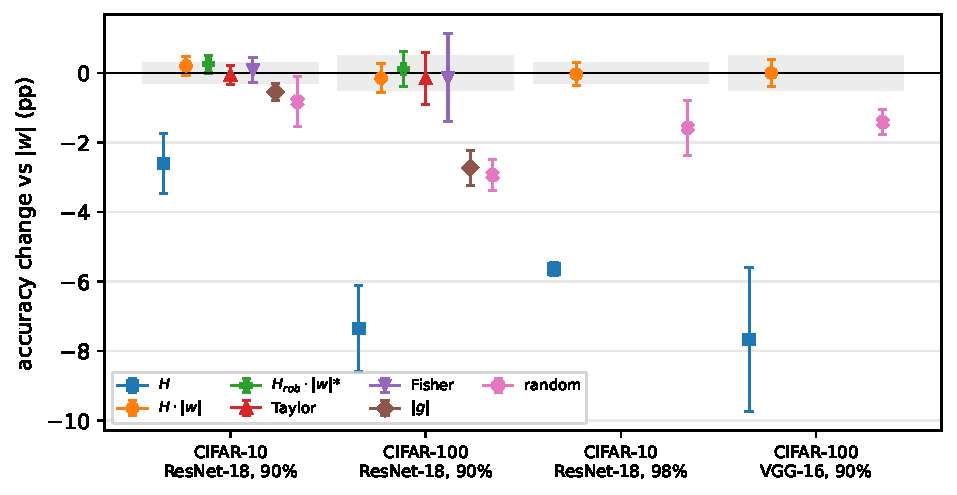
\includegraphics[width=0.9\textwidth]{Figures/penalty_by_regime.pdf}
\caption{Accuracy change of each criterion relative to $|w|$ (95\% Welch CI) in each regime. The grey band is the equivalence margin ($\pm0.3$ points on CIFAR-10, $\pm0.5$ on CIFAR-100). Open marker: exploratory criterion.}
\label{fig:penalty}
\end{figure*}

\paragraph{Difficulty (H3).} Fig.~\ref{fig:penalty} summarises Table~\ref{tab:regimes}. Every criterion that is far from $|w|$ loses more in the harder regimes than on CIFAR-10 at 90\%: entropy alone from $2.6$ to between $5.6$ and $7.7$ points, random from $0.8$ to between $1.4$ and $2.9$, gradient magnitude from $0.5$ to $2.7$. The number of criteria with a significant difference does not rise uniformly (2 of 6 on CIFAR-10 at 90\%, 3 of 6 on CIFAR-100, 1 of 3 at 98\%, 2 of 3 with VGG-16), partly because the secondary regimes test fewer criteria. H3 is supported for the size of the penalties and only partly for their number.

\paragraph{FLOPs.} Criteria that remove the same number of weights remove different amounts of computation, because they allocate the budget differently across layers. On CIFAR-10 at 90\%, $|w|$ removes 74.5\% of the non-zero FLOPs, $H\cdot|w|$ 73.4\%, Taylor and Fisher about 71\%, random 81.5\% and $H$ alone 86.0\%. The two worst criteria remove the most FLOPs, because they prune the early, high-resolution layers more (Fig.~\ref{fig:density}); none of these differences is realised as a speed-up with dense kernels.

\begin{figure*}[t]
\centering
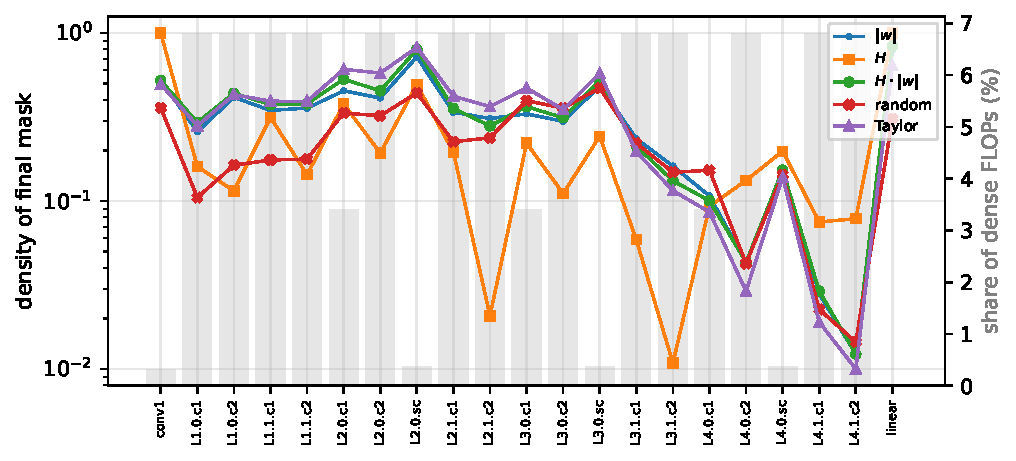
\includegraphics[width=0.9\textwidth]{Figures/layer_density_cifar10_resnet18_s90.pdf}
\caption{Density of the final mask per layer (log scale, mean over seeds) for several criteria, ResNet-18 on CIFAR-10 at 90\% sparsity. Grey bars: each layer's share of the dense FLOPs. All criteria keep the same total number of weights.}
\label{fig:density}
\end{figure*}

\subsection{Allocation or ranking? (H5)}
\label{sec:allocation}

Table~\ref{tab:allocation} repeats the ablation with a layer-uniform allocation, in which no criterion can move budget between layers.

\begin{table*}[t]
\centering
\caption{C0 criteria with global and layer-uniform allocation (CIFAR-10, ResNet-18, 90\%). With uniform allocation every layer keeps the same density, so differences can only come from which weights are dropped inside a layer.}
\label{tab:allocation}
\resizebox{\textwidth}{!}{%
\begin{tabular}{llcccccc}
\toprule
Allocation & Drop criterion & Acc (\%) & $\Delta$ vs $|w|$ [95\% CI] (pp) & $p_{\mathrm{Holm}}$ & Equiv. & FLOPs red.\ sparse (\%) & Seeds \\
\midrule
global & $|w|$ & 95.03 $\pm$ 0.07 & -- & -- & -- & 75.2 $\pm$ 1.5 & 3 \\
global & $H(A)$ & 92.44 $\pm$ 0.40 & -2.59 [-3.55, -1.63] & 0.020 & no & 86.0 $\pm$ 0.7 & 3 \\
global & $H(A)\cdot|w|$ (DEGST) & 95.30 $\pm$ 0.21 & +0.27 [-0.20, +0.74] & 0.288 & no & 73.6 $\pm$ 0.7 & 3 \\
uniform & $|w|$ & 94.43 $\pm$ 0.08 & -- & -- & -- & 90.0 $\pm$ 0.0 & 3 \\
uniform & $H(A)$ & 91.63 $\pm$ 0.37 & -2.80 [-3.67, -1.93] & 0.017 & no & 90.2 $\pm$ 0.0 & 3 \\
uniform & $H(A)\cdot|w|$ (DEGST) & 94.72 $\pm$ 0.23 & +0.29 [-0.21, +0.79] & 0.288 & no & 90.0 $\pm$ 0.0 & 3 \\
\bottomrule
\end{tabular}}
\par\smallskip\footnotesize Mean $\pm$ std over 3 seeds; $^{*}$ marks single-seed cells (no std); -- = not yet run. Accuracy is final-epoch test accuracy. $\Delta$: difference of means to the $|w|$ row of the same block, with its 95\% Welch CI; $p_{\mathrm{Holm}}$: two-sided Welch test, Holm-adjusted over all confirmatory comparisons of the table; Equiv.: TOST at $\pm$0.3 pp (CIFAR-10) / $\pm$0.5 pp (CIFAR-100, Tiny ImageNet), $\alpha$ = 0.05. Exploratory rows are not in the Holm family (unadjusted $p$). Measured sparsity of $H(A)$ (uniform): 90.17--90.33\%, because weights regrown where the gradient is exactly zero (inputs from dead channels) stay zero.
\end{table*}


Entropy alone remains $2.80$ points below $|w|$ ($[-3.67,-1.93]$), compared with $2.59$ points under global allocation, so H5 is not supported: its loss comes from which weights it drops inside each layer, not from the allocation. This also rules out a second explanation suggested by Fig.~\ref{fig:density}: under global allocation, entropy alone keeps the first convolution and the classifier dense but drives two middle layers down to 1--2\% density, close to the per-layer floor. With uniform allocation no layer can be starved in this way, and the loss remains. $H\cdot|w|$ is again not significantly different from $|w|$ ($+0.29$, $[-0.21,+0.79]$). Uniform allocation costs $|w|$ itself $0.6$ points while removing more FLOPs (90\% instead of 75\%). With uniform allocation, entropy alone ends at 90.2--90.3\% measured sparsity instead of 90.0\%: every layer must regrow its own quota, and weights regrown where the gradient is exactly zero (inputs from dead channels) stay zero. This makes its effective budget 2--3\% smaller, far too little to account for a gap of almost three points.

\subsection{How far is each criterion from magnitude? (H4)}
\label{sec:divergence}

Fig.~\ref{fig:divergence} plots each criterion's accuracy change against its divergence from $|w|$.

\begin{figure}[t]
\centering
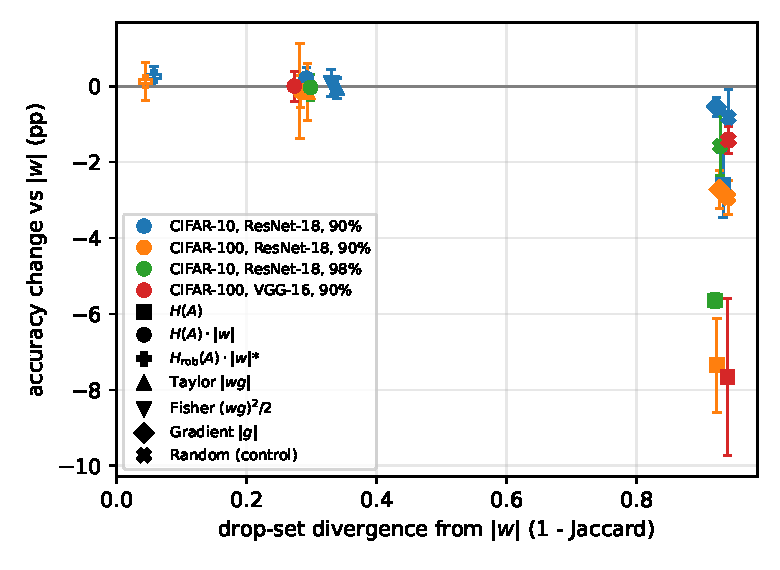
\includegraphics[width=\linewidth]{Figures/divergence_accuracy.pdf}
\caption{Accuracy change relative to $|w|$ (with 95\% CI) against the drop-set divergence $1-J$ from $|w|$, measured by replaying the loop's updates at epochs 50 and 100 (Sec.~\ref{sec:overlap}). Colours: regimes; markers: criteria; open markers: exploratory.}
\label{fig:divergence}
\end{figure}

The pre-specified test supports H4: Spearman $\rho=-0.70$ over the 18 confirmatory points ($p=0.001$). The figure shows, however, that the divergences fall into two clusters rather than along a continuum. $H\cdot|w|$, Taylor and Fisher drop sets differ from that of $|w|$ with divergences between 0.27 and 0.34, and their accuracy changes lie between $-0.15$ and $+0.21$ points, none of them significant. $H$ alone, $|g|$ and random share almost nothing with $|w|$ (divergences 0.92--0.94) and lose between $0.54$ and $7.67$ points. Within that far cluster the divergence is nearly constant while the loss varies fourteen-fold, so the divergence does not explain it. The correlation therefore mostly reflects the near/far split; the points also share regimes and the $|w|$ reference, so the $p$-value is optimistic (post hoc: within-regime $\rho$ is $-0.94$ and $-0.83$ in the two main regimes with six points each, and $-0.50$ in the secondary regimes with three). We read the result as a tolerance rather than a dose--response: the loop absorbs a change of about a third of the dropped weights at no measurable cost, while criteria that ignore magnitude altogether lose accuracy by an amount that depends on the criterion.

\subsection{What the entropy score measures}
\label{sec:what-h}

\paragraph{Entropy alone is worse than random (post hoc).} At the same divergence from $|w|$, entropy alone loses far more than a random drop. Table~\ref{tab:hrandom} compares the two directly.

\begin{table*}[t]
\centering
\caption{Post hoc comparison: drop by entropy alone against random drop, same loop and regrowth. Both drop sets overlap with that of $|w|$ by less than 10\% (Fig.~\ref{fig:divergence}).}
\label{tab:hrandom}
\resizebox{\textwidth}{!}{%
\begin{tabular}{lcccc}
\toprule
Regime & $H(A)$ (\%) & Random (\%) & $\Delta$ $H(A) -$ random [95\% CI] (pp) & $p_{\mathrm{Holm}}$ \\
\midrule
CIFAR-10, ResNet-18, 90\% & 92.44 $\pm$ 0.40 & 94.23 $\pm$ 0.35 & -1.79 [-2.64, -0.93] & 0.009 \\
CIFAR-100, ResNet-18, 90\% & 69.24 $\pm$ 0.57 & 73.65 $\pm$ 0.22 & -4.41 [-5.65, -3.18] & 0.007 \\
CIFAR-10, ResNet-18, 98\% & 88.13 $\pm$ 0.08 & 92.21 $\pm$ 0.35 & -4.07 [-4.89, -3.25] & 0.006 \\
CIFAR-100, VGG-16, 90\% & 66.28 $\pm$ 0.87 & 72.53 $\pm$ 0.18 & -6.25 [-8.29, -4.21] & 0.009 \\
\bottomrule
\end{tabular}}
\par\smallskip\footnotesize Welch tests, Holm-adjusted over the regimes shown. This comparison was not planned before the results; it is reported as a post hoc analysis.
\end{table*}


Entropy alone is worse than random in every regime, by $1.8$ to $6.3$ points ($p_{\mathrm{Holm}}<0.01$). It is not merely uninformative; it is misleading.

\paragraph{Entropy measures sparsity.} In the replay, the entropy of a channel is strongly anti-correlated with its share of exact zeros: Spearman $\rho$ between $-0.61$ and $-0.93$ over all channels after the first layer, at every checkpoint (Fig.~\ref{fig:hsparsity}). After a ReLU, most of a sparse channel's values fall into the first histogram bin, so its entropy is low. Ranking by low entropy therefore removes the weights that read the sparsest channels. That this is worse than random suggests that these channels, silent on most inputs, carry selective, discriminative responses, which a histogram entropy counts as uninformative. The correlation is measured; the interpretation is our explanation of it.

\begin{figure*}[t]
\centering
\IfFileExists{Figures/entropy_vs_sparsity.pdf}{%
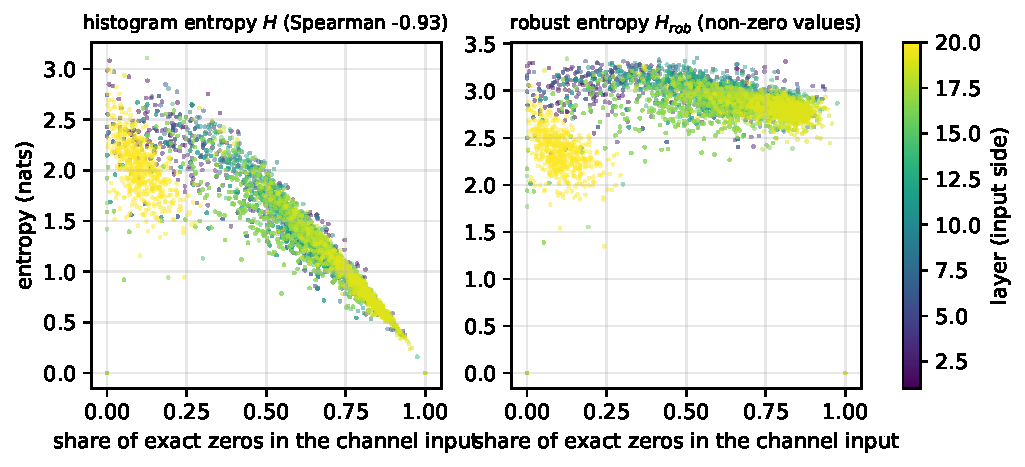
\includegraphics[width=0.9\textwidth]{Figures/entropy_vs_sparsity.pdf}}{%
\fbox{\parbox{0.8\textwidth}{\centering\vspace{2em}Figure pending: run \texttt{analysis/score\_overlap.py} on the epoch-50 checkpoint with \texttt{--out-dir results/analysis\_channels}, then \texttt{aggregate.py}.\vspace{2em}}}}
\caption{Per-channel entropy of the input of every layer after the first against the share of exact zeros in that input, ResNet-18 on CIFAR-100 at 90\% sparsity, epoch 50. Left: the histogram entropy used by the criteria. Right: the robust estimate over non-zero values. Colour: layer depth.}
\label{fig:hsparsity}
\end{figure*}

\paragraph{A robust estimate (exploratory).} $H_{\mathrm{rob}}\cdot|w|$ removes the zeros and outliers from the estimate. Its drop sets are almost those of $|w|$ (divergence 0.04--0.07): once zeros are excluded, the entropy varies little across the channels of a layer and hardly changes the ranking. Its difference to $|w|$ is $+0.26$ points on CIFAR-10 ($[+0.01,+0.52]$, unadjusted $p=0.047$) and $+0.12$ on CIFAR-100 ($[-0.39,+0.63]$). Given how little it changes the drop sets and that the result does not repeat on CIFAR-100, we do not interpret the CIFAR-10 difference.
